\section{交替极小化}
\label{sec:block-alternating}

前面的块多半是单个坐标或一小组坐标。有些问题的变量天然分成少数几组，每组固定其余后都容易解。沿用精确块更新依次解这几组，能得到什么，又在哪里止步？

\term{交替极小化}（alternating minimization）就是块数较少时的精确BCD，它是组织条件求解的一种方式，并不是一类新的优化理论。下面以矩阵分解为主例，并区分三个常被混在一起的性质。分别凸使每个条件子问题容易解；块解唯一使迭代有确定含义，并支撑极限分析；联合凸才能把驻点推到全局最优。

\subsection{交替最小二乘（ALS）}
\label{sec:block-als}

\paragraph{主要思想}
回到矩阵分解问题
\begin{equation}
 \min_{\bm{U},\bm{V}}\ \Phi(\bm{U},\bm{V})=\lVert\bm{Y}-\bm{U}\bm{V}^\top\rVert_F^2 .
 \label{eq:block-factorization}
\end{equation}
它关于$(\bm{U},\bm{V})$联合起来不是凸函数，但固定一个因子，另一个因子就是线性最小二乘。\term{交替最小二乘}（alternating least squares，ALS）轮流解这两个问题。

固定$\bm{V}$，目标按行拆开。记$\bm{Y}$的第$i$行为$\bm{y}_i^\top$，$\bm{U}$的第$i$行为$\bm{u}_i^\top$，则
\[
 \lVert\bm{Y}-\bm{U}\bm{V}^\top\rVert_F^2=\sum_{i=1}^{p}\lVert\bm{y}_i-\bm{V}\bm{u}_i\rVert_2^2 .
\]
每一行都是一个系数矩阵为$\bm{V}$的最小二乘问题，图~\ref{fig:block-als-structure}(a)标出了这种按行的结构。

\begin{BookInlineFigure}
  \centering
  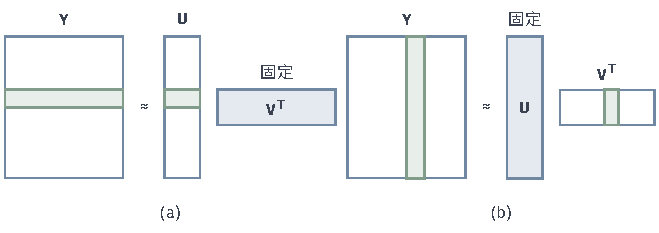
\includegraphics[width=110mm]{figures/05-optimization/04-block-optimization/tikz/block-als-structure/figure.pdf}
  \caption{ALS的两个半步。(a)固定$\bm{V}^\top$（蓝）时，$\bm{Y}$的每一行只依赖$\bm{U}$的对应行（绿），问题拆成$p$个共用系数矩阵的最小二乘。(b)固定$\bm{U}$（蓝）时，$\bm{Y}$的每一列只依赖$\bm{V}^\top$的对应列，同样拆开。}
  \label{fig:block-als-structure}
\end{BookInlineFigure}

对$\bm{u}_i$求导并把$p$行合起来，得到正规方程
\[
 \bm{U}\bm{V}^\top\bm{V}=\bm{Y}\bm{V}.
\]
若$\bm{V}$满列秩，$\bm{V}^\top\bm{V}$可逆，解唯一：
\begin{equation}
 \bm{U}^{+}=\bm{Y}\bm{V}(\bm{V}^\top\bm{V})^{-1}.
 \label{eq:block-als-u}
\end{equation}
同理，固定$\bm{U}$且$\bm{U}$满列秩时，
\begin{equation}
 \bm{V}^{+}=\bm{Y}^\top\bm{U}(\bm{U}^\top\bm{U})^{-1}.
 \label{eq:block-als-v}
\end{equation}

\paragraph{秩亏时的选解}
若$\bm{V}$不满列秩，正规方程有无穷多解。此时要规定选哪一个，常用的是Frobenius范数最小的解
\[
 \bm{U}^{+}=\bm{Y}\bm{V}(\bm{V}^\top\bm{V})^{\dagger},
\]
其中$\dagger$表示伪逆。比如$\bm{V}=\bm{0}$时，任何$\bm{U}$都使目标等于$\lVert\bm{Y}\rVert_F^2$，这个规则选$\bm{U}=\bm{0}$。

\paragraph{三种计算方式}
式~\eqref{eq:block-als-u}要解的是$p$个右端不同、系数相同的方程。系数矩阵是同一个，逐行重新分解是浪费，分解只需做一次。设$\bm{V}\in\mathbb{R}^{q\times r}$，$\bm{Y}$稠密，一个半步的主要运算是：
\begin{itemize}
 \item 形成$\bm{V}^\top\bm{V}$，约$qr^2$；形成$\bm{Y}\bm{V}$，约$pqr$。
 \item 做一次Cholesky分解，约$r^3/3$。
 \item 对$p$行各做一次前代回代，约$2pr^2$。
\end{itemize}
$\bm{Y}$稀疏时第二项换成$r$乘以非零元数。分解的条件数是$\bm{V}$的条件数的平方，$\bm{V}$接近秩亏时，改用$\bm{V}$的QR分解更稳定，但一次分解的运算量约为$2qr^2$。

加入正则项$\gamma(\lVert\bm{U}\rVert_F^2+\lVert\bm{V}\rVert_F^2)$，$\gamma>0$，后，系数矩阵变成严格正定，子问题总有唯一解：
\begin{equation}
 \bm{U}^{+}=\bm{Y}\bm{V}(\bm{V}^\top\bm{V}+\gamma\bm{I})^{-1}.
 \label{eq:block-als-ridge}
\end{equation}
秩亏的麻烦由此消除，代价是目标改变了，解被拉向零。

\paragraph{完整目标不增}
两个半步各是一次精确块更新，由引理~\ref{lem:block-exact-descent}，连起来就是
\begin{equation}
 \Phi(\bm{U}^{(t+1)},\bm{V}^{(t+1)})\leq\Phi(\bm{U}^{(t+1)},\bm{V}^{(t)})\leq\Phi(\bm{U}^{(t)},\bm{V}^{(t)}).
 \label{eq:block-als-monotone}
\end{equation}
目标有下界$0$，目标值序列因此收敛。注意这只说明目标值收敛，并不说明因子本身收敛，因为$(c\bm{U},\bm{V}/c)$与$(\bm{U},\bm{V})$有相同的目标值，因子的尺度不由目标决定。

\needspace{6\baselineskip}
\paragraph{变量}
\begin{itemize}
 \item $\bm{U}\in\mathbb{R}^{p\times r}$，$\bm{V}\in\mathbb{R}^{q\times r}$：两个因子。
 \item $\bm{Y}\in\mathbb{R}^{p\times q}$：数据矩阵，只读。
\end{itemize}

\paragraph{初始化}
选定秩$r$，随机初始化$\bm{V}^{(0)}$。下面用一个$r=1$的例子，因子都是向量，记为$\bm{u},\bm{v}$：
\[
 \bm{Y}=\begin{bmatrix}3&1\\1&3\end{bmatrix},\qquad \bm{v}^{(0)}=(1,0),
\]
于是$\lVert\bm{Y}\rVert_F^2=20$。

\needspace{6\baselineskip}
\paragraph{每轮更新}
在第$t$轮：
\begin{enumerate}
 \item \textbf{更新$\bm{U}$。}由式~\eqref{eq:block-als-u}计算。例中$\bm{u}=\bm{Y}\bm{v}/\lVert\bm{v}\rVert_2^2$，第一轮
 \[
  \bm{u}^{(1)}=(3,1),\qquad \Phi=10 .
 \]
 \item \textbf{更新$\bm{V}$。}由式~\eqref{eq:block-als-v}计算。例中$\bm{v}=\bm{Y}^\top\bm{u}/\lVert\bm{u}\rVert_2^2$，第一轮
 \[
  \bm{v}^{(1)}=\frac{(10,6)}{10}=(1,0.6),\qquad \Phi=6.4 .
 \]

 第二轮用$\bm{v}^{(1)}$计算，$\lVert\bm{v}^{(1)}\rVert_2^2=1.36$，于是
 \[
  \bm{u}^{(2)}=\frac{(3.6,2.8)}{1.36}\approx(2.647,2.059),\qquad \Phi\approx4.706 .
 \]
 再更新$\bm{v}$，$\lVert\bm{u}^{(2)}\rVert_2^2\approx11.246$，于是
 \[
  \bm{v}^{(2)}\approx(0.889,0.785),\qquad \Phi\approx4.185 .
 \]
 \item \textbf{检查停止。}目标值的相对下降或因子的相对变化小于容差时结束。
\end{enumerate}

第二轮的$\bm{v}$两个分量之比已经接近$1$，最终得到$\bm{u},\bm{v}$都平行于$(1,1)$，目标值趋于$4$。这个$4$正是$\bm{Y}$的第二个奇异值的平方，由矩阵逼近的结论，它是所有秩$1$逼近的最小误差；相关的定理可参考\BookChapterRef{chap:matrix-approximation}{卷二第18章“矩阵逼近”}。

这个例子中，交替更新实际上是幂迭代。把两个半步合起来，$\bm{v}$的新方向正比于$\bm{Y}^\top\bm{Y}\bm{v}$，$\bm{Y}^\top\bm{Y}$的特征值是$16$和$4$，所以偏离主方向的分量每轮缩小到$\tfrac14$。

图~\ref{fig:block-als-descent}(a)是这个例子的目标值阶梯，(b)取一个噪声较大的$40\times25$矩阵，从不同的随机起点出发，都很快接近截断奇异值分解给出的最优值。一般情形下ALS并不总能这样达到全局最优，下一小节就是反例。

\begin{BookInlineFigure}
  \centering
  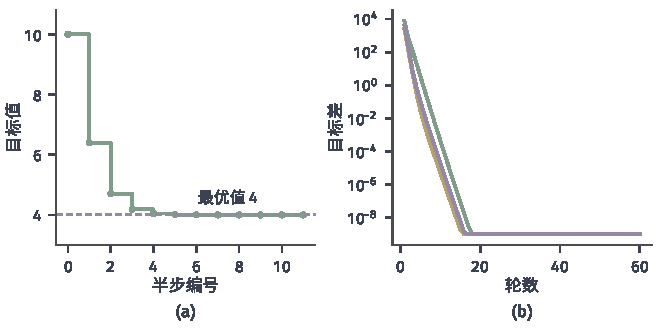
\includegraphics[width=112mm]{figures/05-optimization/04-block-optimization/matplotlib/block-als-descent/figure.pdf}
  \caption{ALS的目标值。(a)文中$2\times2$的例子，每半步记录一次，绿色阶梯单调下降，紫色虚线是最优秩$1$误差$4$。(b)$40\times25$的矩阵（秩$3$信号加噪声），$r=3$，三种颜色是三个随机起点，纵轴是目标值与截断奇异值分解最优值之差，下方平台是绘图的截断值。}
  \label{fig:block-als-descent}
\end{BookInlineFigure}

\subsection{逐块最优的局限}
\label{sec:block-limits}

\paragraph{停在鞍点的例子}
每一步都精确解出了条件子问题，最后能到全局最优吗？考虑带正则的双线性目标，$0<\rho<1$：
\begin{equation}
 \Phi_\rho(u,v)=\frac12(uv-1)^2+\frac{\rho}{2}(u^2+v^2).
 \label{eq:block-saddle-example}
\end{equation}
固定$v$，它是$u$的二次函数，$u^2$的系数是$(v^2+\rho)/2>0$，所以条件子问题有唯一解。令偏导数为零，得到
\begin{equation}
 u=\frac{v}{v^2+\rho},\qquad v=\frac{u}{u^2+\rho}.
 \label{eq:block-saddle-update}
\end{equation}
这里两个条件子问题都严格凸、解唯一，看上去已经是最好的情形了。

下面取$\rho=0.36$。全局最小点在$u=v=\pm\sqrt{1-\rho}=\pm0.8$，最小值是$\rho-\rho^2/2=0.2952$。从$v=0.6$出发，迭代是
\[
 u=0.8333,\quad v=0.7903,\quad u=0.8027,\quad v=0.7992,\quad u=0.8002,
\]
目标值从$0.3148$很快降到最小值附近。

现在换一个起点：$u=v=0$。由式~\eqref{eq:block-saddle-update}，两个更新都给出$0$，迭代永远停在原点，目标值是$\tfrac12$。

原点是什么样的点？两个偏导数都是$0$，它是驻点。它的Hessian是
\[
 \begin{bmatrix}\rho&-1\\-1&\rho\end{bmatrix},
\]
特征值$\rho-1=-0.64$和$\rho+1=1.36$一负一正，所以原点是鞍点，不是极小点。图~\ref{fig:block-saddle}画出了这一点。

\begin{BookInlineFigure}
  \centering
  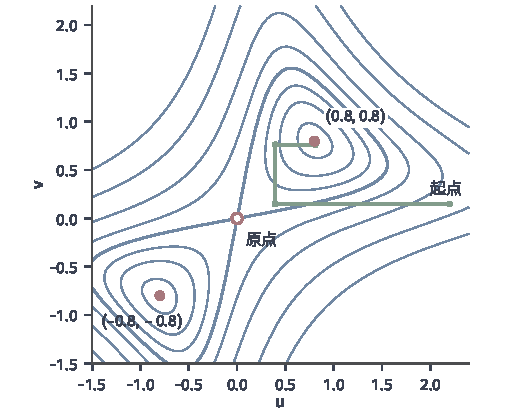
\includegraphics[width=88mm]{figures/05-optimization/04-block-optimization/matplotlib/block-saddle/figure.pdf}
  \caption{交替极小化与鞍点。$\Phi_\rho$的等高线（$\rho=0.36$），加粗的一条是$\Phi_\rho=\tfrac12$，正好穿过原点。绿色折线从$(2.2,0.15)$出发，收敛到红点$(0.8,0.8)$。红色空心点是原点：两个条件子问题的解都是$0$，从这里出发的迭代不动，而沿Hessian的负特征方向目标还能下降。}
  \label{fig:block-saddle}
\end{BookInlineFigure}

原点并不吸引路径。在原点附近$u\approx v/\rho$，$v\approx u/\rho$，一轮下来$v$约放大$1/\rho^2\approx7.7$倍，所以只要$v$不恰好为零，迭代就会被推开。图中的绿线就从靠近原点的横线上逃开了。不过这种稳定性分析需要另外的工作，逐块最优这个性质本身不能排除鞍点。

\paragraph{三个层次的对比}
再把第~\ref{sec:block-coupling}小节的反例放进来，就能看清三个不同的层次。下表中，“逐块最优”指对每个块，当前点都是条件子问题的最优解。

\begin{BookInlineTable}
\centering
\begin{tabular}{lll}
\toprule
情形 & 逐块最优 $\Rightarrow$ 驻点？ & 驻点 $\Rightarrow$ 全局最优？\\
\midrule
光滑非凸（例~\eqref{eq:block-saddle-example}） & 是 & 否，原点是鞍点\\
不可分（例~\eqref{eq:block-nonsmooth-example}） & 否，原点不是驻点 & 凸时为是\\
光滑加可分凸项，联合凸 & 是 & 是\\
\bottomrule
\end{tabular}
\end{BookInlineTable}

第一列的结论：对光滑目标，每个块的偏梯度为零，合起来就是整个梯度为零，所以逐块最优蕴含驻点。可分的非光滑项也可以这样合起来。不可分的非光滑项不行，这正是例~\eqref{eq:block-nonsmooth-example}停滞的原因。

第二列的结论：驻点推出全局最优需要联合凸性，只是分别凸还不够。在例~\eqref{eq:block-saddle-example}中，固定任一变量时函数都凸，联合起来却不凸。

\paragraph{联合凸时的结论}
联合凸性加上可分结构后，上述三个层次重合，这时逐块最优就是全局最优。

\begin{lemma}[联合凸时逐块最优即全局最优]
\label{lem:block-joint-convex}
设$F=f+\sum_Jg_J$，$f$在$\mathbb{R}^n$上凸且可微，各$g_J$是适当凸函数。若$\bar{\bm{x}}$满足$F(\bar{\bm{x}})<+\infty$，且对每个块$J$，$\bar{\bm{x}}_J$是块$J$条件子问题的最优解，则$\bar{\bm{x}}$是$F$的全局最小点。
\end{lemma}

\begin{proof}
取任意$\bm{y}\in\mathbb{R}^n$，固定一块$J$，令$\bm{h}=\bm{y}_J-\bar{\bm{x}}_J$。对$s\in(0,1]$，由块最优性，
\[
 f(\bar{\bm{x}}+s\bm{U}_J\bm{h})+g_J(\bar{\bm{x}}_J+s\bm{h})\geq f(\bar{\bm{x}})+g_J(\bar{\bm{x}}_J).
\]

由$g_J$的凸性，
\[
 g_J(\bar{\bm{x}}_J+s\bm{h})\leq(1-s)g_J(\bar{\bm{x}}_J)+sg_J(\bm{y}_J),
\]
代入并整理得
\[
 \frac{f(\bar{\bm{x}}+s\bm{U}_J\bm{h})-f(\bar{\bm{x}})}{s}+g_J(\bm{y}_J)-g_J(\bar{\bm{x}}_J)\geq0 .
\]
令$s\downarrow0$，第一项趋于$\langle\nabla_Jf(\bar{\bm{x}}),\bm{h}\rangle$，于是
\[
 \langle\nabla_Jf(\bar{\bm{x}}),\bm{y}_J-\bar{\bm{x}}_J\rangle+g_J(\bm{y}_J)-g_J(\bar{\bm{x}}_J)\geq0 .
\]

对所有块求和。$f$是凸函数，所以
\[
 f(\bm{y})\geq f(\bar{\bm{x}})+\langle\nabla f(\bar{\bm{x}}),\bm{y}-\bar{\bm{x}}\rangle,
\]
于是
\[
 \begin{aligned}
 F(\bm{y})-F(\bar{\bm{x}})
 &\geq\langle\nabla f(\bar{\bm{x}}),\bm{y}-\bar{\bm{x}}\rangle+\sum_J\bigl(g_J(\bm{y}_J)-g_J(\bar{\bm{x}}_J)\bigr)\\
 &\geq0 .
 \end{aligned}
\]
\end{proof}

证明中用到可分结构的地方是把各块的不等式相加。这正好解释了例~\eqref{eq:block-nonsmooth-example}为什么失败：它的非光滑项不能写成$\sum_Jg_J(\bm{x}_J)$，两块的不等式加不到一起。
